\documentclass[10pt,a4paper]{article}
\usepackage[utf8]{inputenc}
\usepackage{amsmath}
\usepackage{amsfonts}
\usepackage{amssymb}
\usepackage{float}
\newcommand\tab[1][1cm]{\hspace*{#1}}
\usepackage{graphicx}
\usepackage{scrextend}
\usepackage{wrapfig}
\usepackage{enumitem}
\author{Konrad Cybulski, Julian Kardis, Matteo Batelic}
\title{Understanding Trends in Global Terrorism}
\begin{document}
\begin{titlepage}
    \begin{center}
        \vspace*{1cm}
        
        \LARGE
        \textbf{Understanding Trends in Global Terrorism}
        
        \vspace{4cm}
        
		\Large 
        
        \textbf{Konrad Cybulski, Julian Kardis, Matteo Batelic}
        
        
        \LARGE
        \vspace{2cm}

        
        
        \vfill
        
        
        
        Final report \\
        FIT2083 Research Project
        
        
        
\includegraphics[width=0.4\textwidth]{monash-university-logo.png}
              
        
        \large
        Faculty of Information Technology\\
        Monash University\\
        Australia\\
        24/10/2016
        
    \end{center}
\end{titlepage}

\pagebreak
\tableofcontents
\pagebreak

\section{Abstract} 
Terrorism data analysis is vast and complicated, there are multiple  types of terrorism and the traits and motivation can differ rapidly in each region of the world. In this exploration study, the connection between media coverage and terrorism attack/ deaths, the different trends of attack methods, terrorism trends over time and comparing rates of success of terrorism attacks through different regions of the world will be analysed and contrasted to uncover trends and highlight further research paths that can be studied.  

\section{Introduction} 
Terrorism is vast and complicated, being caused and provoked by numerous reasons.  This exploratory study aims to understand broad trends in global and country specific reigens. Utilising the ‘Global Terrorism Database’ from (START, 2016) consisting of ‘More than 150,000 terrorist attacks worldwide’ from 1970 to 2015 we aim to understand trends in countries with high rates of terrorism, methods of attacks, understanding rates of success in terror attacks and by utilising a count of both total and terrorism specific  articles produced by The New York Times newspaper we aim to answer if the recent influx of news articles due to the new accessibility of news has an effect on terrorism trends in America.

\section{Background}
		\subsection{The common issues in terrorism research}
The scientific study of terrorism is plagued by three common issues throughout the literature.
			\subsubsection{Issue One: Defining Terrorism}
There is no universal agreement for a single definition of terrorism (Charters, 1989). This makes conducting research on terrorism problematic, as the definition of terrorism being used often depends upon the perspective the user is taking (Hill, 2016).   \\\\

A clear example of this can be seen within the different agencies of the US government. The US Department of State (22 U.S Code, 2016), The US Federal Emergency Management Agency (FEMA, 2013), The Federal Bureau of Investigations (FBI, 2002) and the U.S Department of Defense (DoD, 2010) all have their own definitions of terrorism due to their departments differing priorities regarding terrorism.    \\\\



			\subsubsection{Issue Two: A Lack of Objective Data on Terrorism}

Due to terrorism being a furtive activity by nature, terrorists are unlikely to report their activities, and in the rare cases they do, are usually doing so to drive factually dubious propaganda (Merari, 2007).  This is compounded by the fact many targets of terrorist attacks are governments, businesses or organizations. Frequently these targets are not interested in providing objective data about the attack due to having their own agenda (Lafree \& Dugan, 2007). \\\\


			\subsubsection{The Third Common Issue: A lack of research to build upon}
The research of terrorism has largely depended on a small pool of active researchers. (Silke, 2008). Although since 9/11, papers in the field of terrorism have tripled, terrorism research is still lagging behind other similar fields of research, such as criminology (Sheehan, 2012).

		\subsection{Addressing the Common Issues}
START has attempted to deal with these common issues by introducing several assumptions into their database.\\\\

To address the lack of a common definition for terrorism, START use a modular criterion for their data, composed of the components of several commonly used definitions. An attack must meet several criteria to be included in the database (START, 2016). This allows the components of several commonly used definitions to be used in conjunction.  START have elected to exclude state sponsored terrorism, even though it meets the criteria. (START GTD, 2017).\\\\

In regards to the issue of objective data, START rely exclusively on media reported incidents that meet their inclusion criteria. START includes failed attacks but omit failed or foiled plots, due to their underreporting (START, 2016).  \\\\

To address a lack of terrorism research to build upon, START have made their data set open source. This introduced the additional problem that database accuracy is dependent on the accuracy of mainstream media reports, and may be biased in favour of the most newsworthy forms of terrorism (START GTD, 2017).

\subsection{Methodological Issues within the GTD}

The data collection methods of the GTD have shifted over the years causing some inconsistencies within the data (START, 2016). This in part is explained by the fact that the groups collecting the data have changed, as well as an extended period of inactivity in the collection of data (LaFree, Dugan, \& Scott, 2006). The following is the summation of the major discrepancies.
\\\\

\textbf{1970 - 1997 }\\\\
The data was initially collected by PGIS from 1970-1997 by recording events reported by the media. (START, 2016)\\\\

\textbf{1993}\\\\
The entire year of 1993 is missing due to a clerical error (LaFree, Dugan, \& Scott, 2006). The current data was retroactively added.
\\\\

\textbf{1997 - 2008}\\\\
The GTD was discontinued between 1997 to 2008. It is for this reason there is a decline in data between 1998 and 2008. All records between this period were collected retroactively in 2008 (LaFree, 2010).
\\\\

\textbf{2012 - Present}\\\\
In 2012 START moved their base of operations to the University of Maryland, where they began to handle data collection locally, instead of through vendors (START, 2016). This change created a spike in the frequency of suicide attacks between 2011 and 2012 that was not observant in similar databases, such as Chicago Project on Security and Terrorism’s Suicide Attack Database (CPOST, 2016).
\\\\

\begin{center}
\begin{figure}[h!]
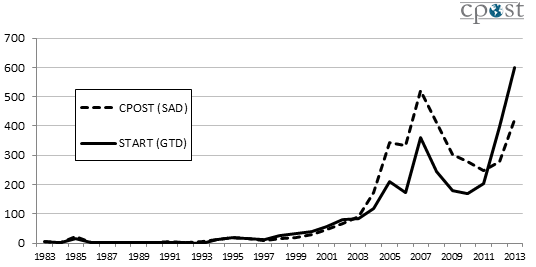
\includegraphics[width=0.9\textwidth]{backgroundpic1.png}
\caption{Comparison of terrorist suicide attacks between CPOST’s Suicide Attack Database and START’s Global Terrorism Database. The START database shows a statistically significant growth difference between 2011 and 2012}
\end{figure}
\end{center}

START has drawn criticism and been accused of politicizing their data (Pape, Kevin, Bauer, \& Jenkins, 2014). START dispute this, and cite their change from vendor based data collection to local based data collection as the reason for this increase in attacks in their data. (START GTD, 2017)

\subsection{START’s Response to Criticism}

In response to these issues, START has publicly stated that differences in trends before and after 1997, before and after 2008, and before and after 2012, can be, at least partially contributed to their data collection methodologies. START recommend any research using GTD data should adjust for these differences (START GTD, 2017). They make no recommendation for the year of 1993.


\begin{center}
\begin{figure}[h!]
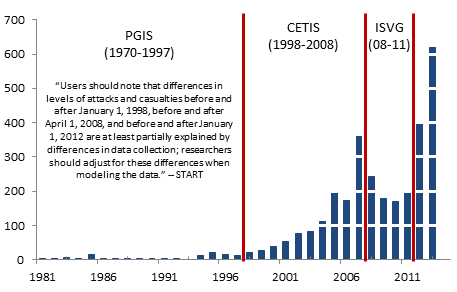
\includegraphics[width=0.9\textwidth]{backgroundpic2.png}
\caption{Critical methodology changes in the GTD. 
The graph shows terrorist attacks per year extracted from the GTD. The years data gathering methodology were changed are indicated by the red lines and labeled with  the organization responsible for the gathering of data for the GTD at the time.
}
\end{figure}
\end{center}

\section{Method}
\subsection{Data}
The database used in this investigation comes from the Global Terrorism Database (GTD) (START, 2016) with 156,749 listings of successful and failed terrorist attacks around the world between 1970 and 2015. With additionally 137 variables including date, country, latitude/longitude, number of perpetrators, number of deaths as a result of the attack, number of injuries, method of attack (bombing, armed assault, etc.) as well as many others. Due to the extensive nature of the database, this investigation aims to understand trends in a select number of these variables. These variables include attack types, deaths, number of attacks, number of successful attacks, and country of attack. In order to understand country specific and global trends in terrorism, the data will be explored not only as a whole, but as a series of subsets of the GTD grouped by country as well as a series of country clusters.
\\\\

\subsection{Analysis}
The methods used to analyse the GTD involved for the most part an analysis of a number of time series'. In order to understand trends of not only single countries, but groups of countries as well as terrorism on a global scale, the groups and countries used were determined in the following way. The country clusters investigated were made up of three groups, typically Western and first world countries (United States, Canada, Australia, France, Finland, Russia, etc.), the six countries with the overall highest number of deaths due to terrorist activity between 1970 and 2015 (which is determined by data from the GTD), and a more in depth look solely at trends in the United States.
\\\\
All three groups are investigated with regard to deaths due to terrorist activity, number of attacks, type of attack and rate of success for a given attack. However the United States is not only subject to investigation into these variables, but using data from the \textit{New York Times}, investigated with regard to possible relationships between the media's coverage of terrorism and rates of attacks and methods of attacks.


\section{Results}
The results produced as outlined by the \textit{Methods} section are below grouped by the variable investigated. These sections include investigation into:\\
\begin{itemize}
\item The relationship between \textit{New York Times} terrorism coverage and United States related terrorism activity.
\item Trends in method of attack in numerous geographical region
\item Terrorism trends over time
\item Rates of success in terrorist attacks 

\end{itemize}

\begin{center}
\begin{figure}[H]		
	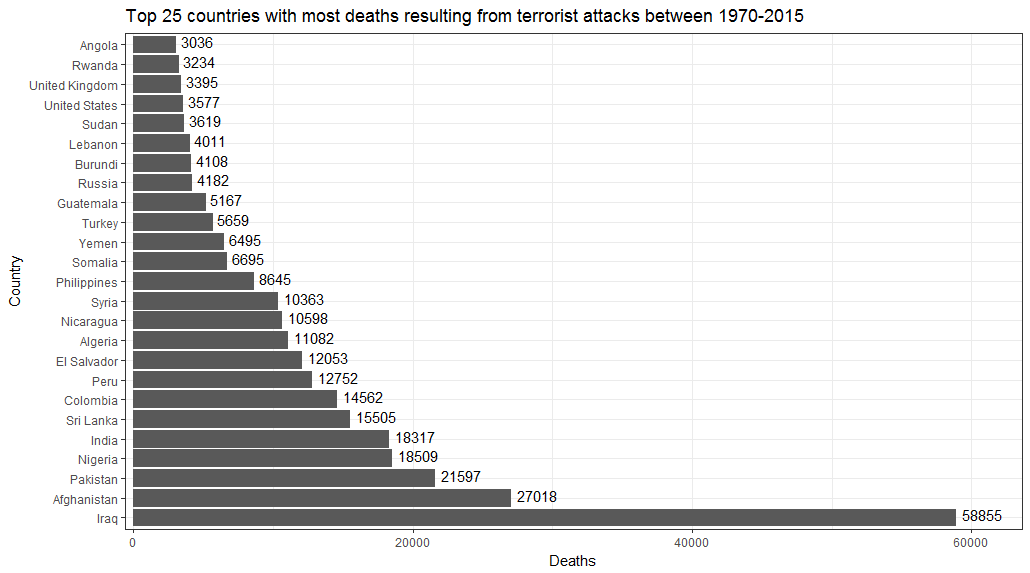
\includegraphics[width=0.8\textwidth]{Plots/Top25countriesbydeaths.png}
	\caption{Top 25 countries by number of deaths resulting from terrorism.}
\end{figure}
\end{center}

\subsection{Terrorism coverage in the United States news data}

\begin{center}
\begin{figure}[H]
		
	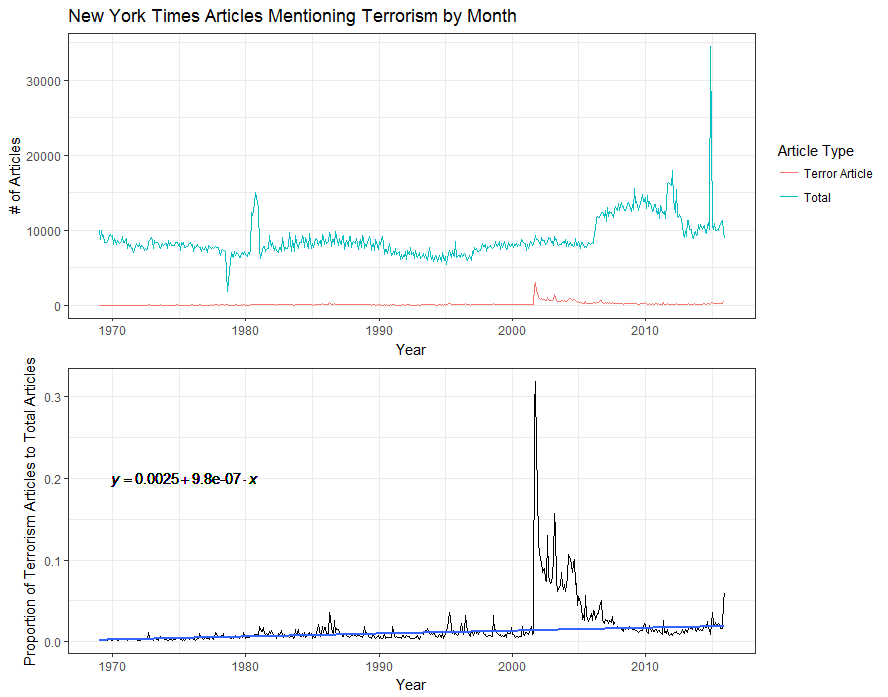
\includegraphics[width=0.8\textwidth]{Plots/NewsData/ArticlesByMonth.png}
	\caption{(Top) New York Times article count and terrorism article count by month. (Bottom) Proportion of terrorism related articles to total articles by month. This is fitted with a robust linear model in order to gain a general overview of possible temporal trends.}
\end{figure}

\begin{figure}[H]
	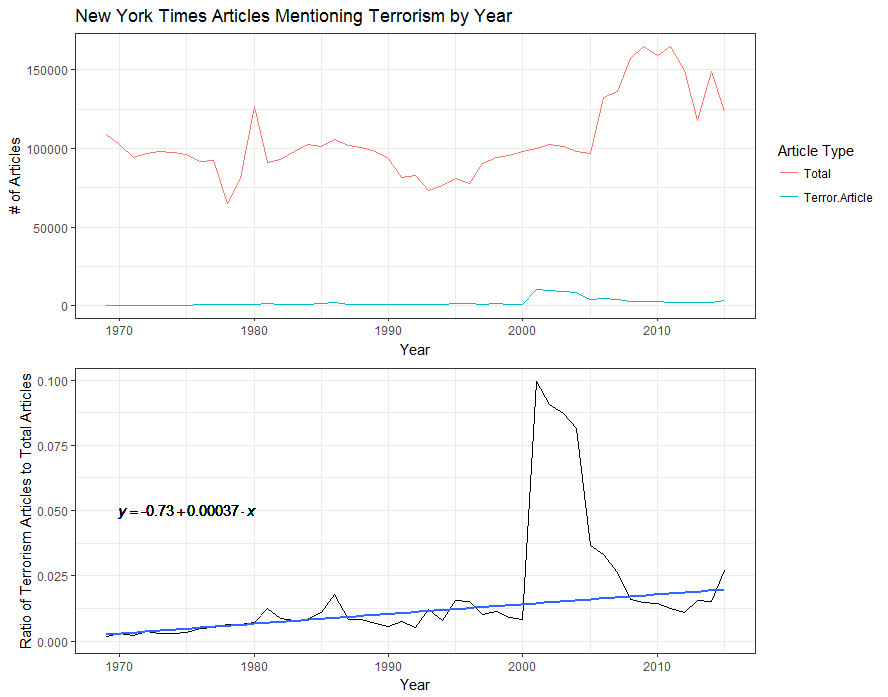
\includegraphics[width=0.8\textwidth]{Plots/NewsData/ArticlesByYear.png}
	\caption{(Top) New York Times article count and terrorism article count by year. 
	(Bottom) Proportion of terrorism related articles to total articles by year. This is fitted with a robust linear model in order to gain a general overview of possible temporal trends.}
\end{figure}

\begin{figure}[H]
	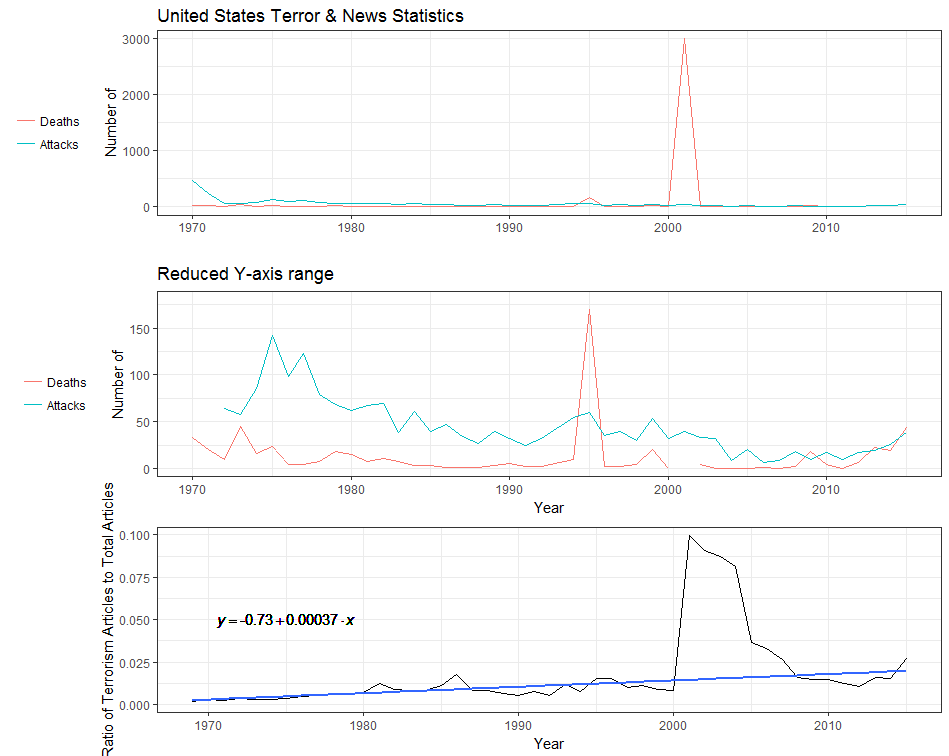
\includegraphics[width=0.8\textwidth]{Plots/NewsData/AttackNewsData.png}
	\caption{(Top) United states deaths and attacks due to terrorism by year. 
	(Middle) United states deaths and attacks due to terrorism by year with a reduced Y-axis range. 
	(Bottom) Proportion of terrorism related articles to total articles by year. This is fitted with a robust linear model in order to gain a general overview of possible temporal trends.}
\end{figure}
\end{center}

\subsection{Method of Attack}

\begin{center}
\begin{figure}[H]
	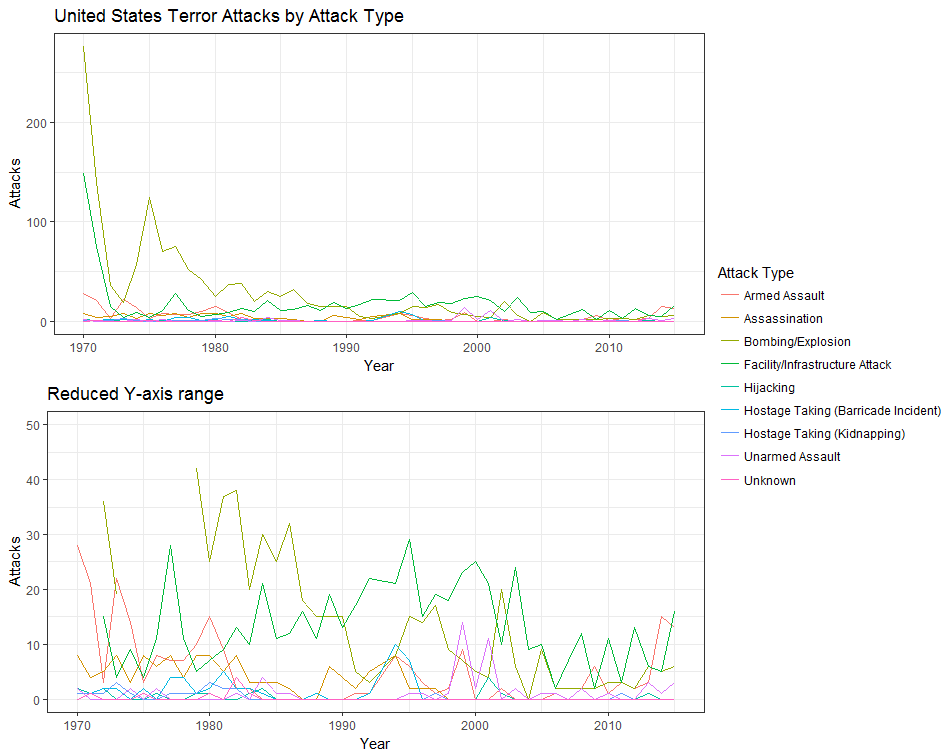
\includegraphics[width=0.8\textwidth]{Plots/AttackType/Attacks.png}
	\caption{United States terror Attacks by Attack Type by year.}
\end{figure}

\begin{figure}[H]
	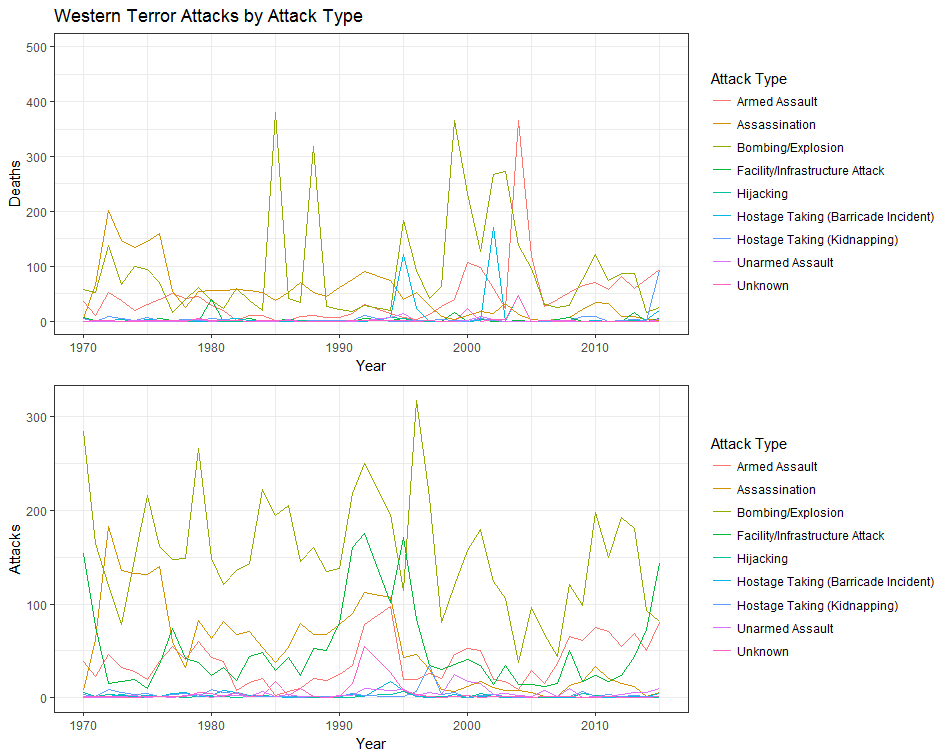
\includegraphics[width=0.8\textwidth]{Plots/AttackType/AttackTypeWesternCountries.png}
	\caption{Western Terror Attacks by Attack Type by year.}
\end{figure}

\begin{figure}[H]
	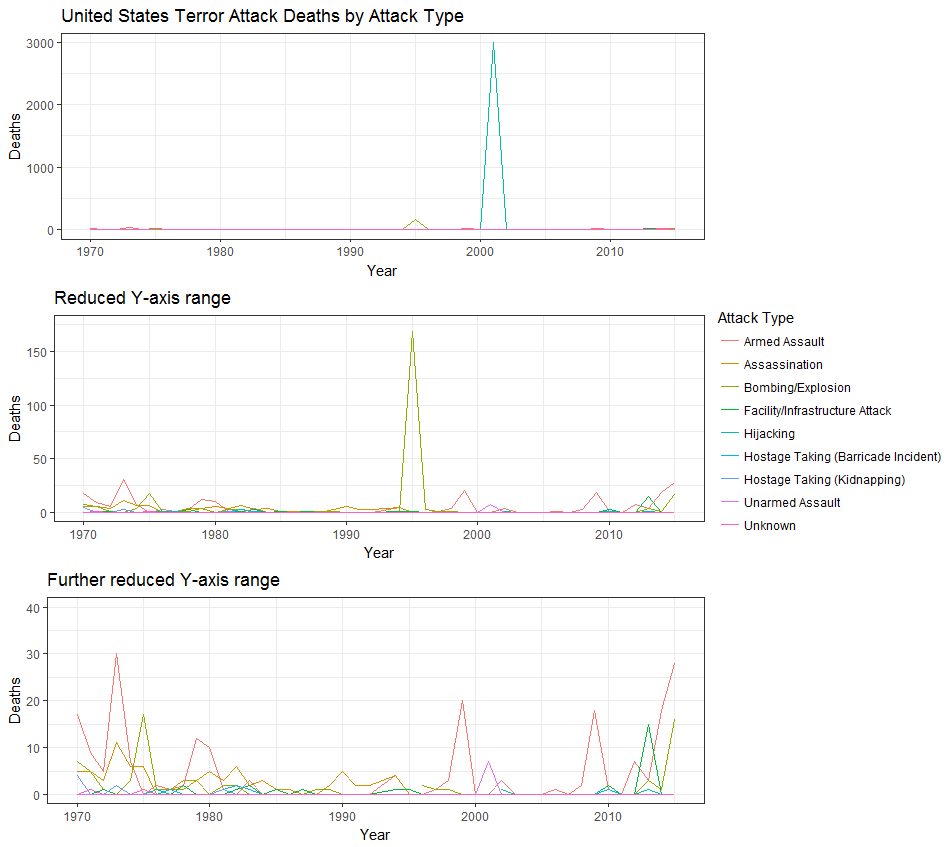
\includegraphics[width=0.8\textwidth]{Plots/AttackType/Deaths.png}
	\caption{United States terror Attack Deaths by Attack Type by year.}
\end{figure}

\begin{figure}[H]
	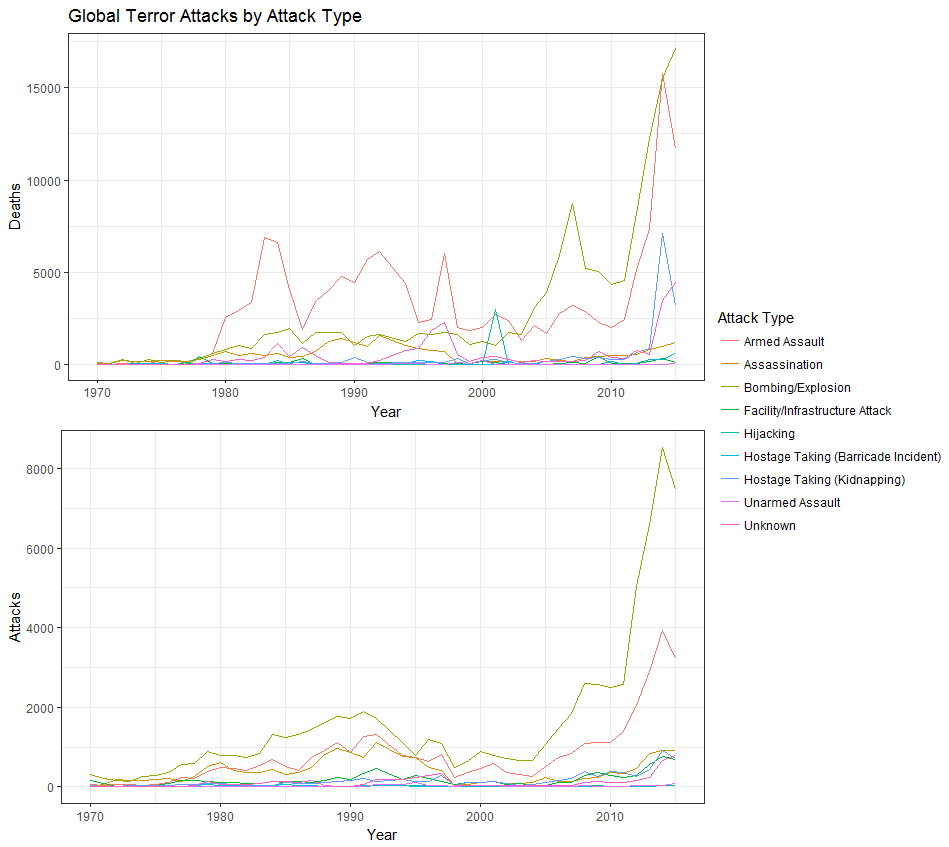
\includegraphics[width=0.8\textwidth]{Plots/AttackType/Global.png}
	\caption{Global Terror Attacks by Attack Type by year.}
\end{figure}

\begin{figure}[H]
	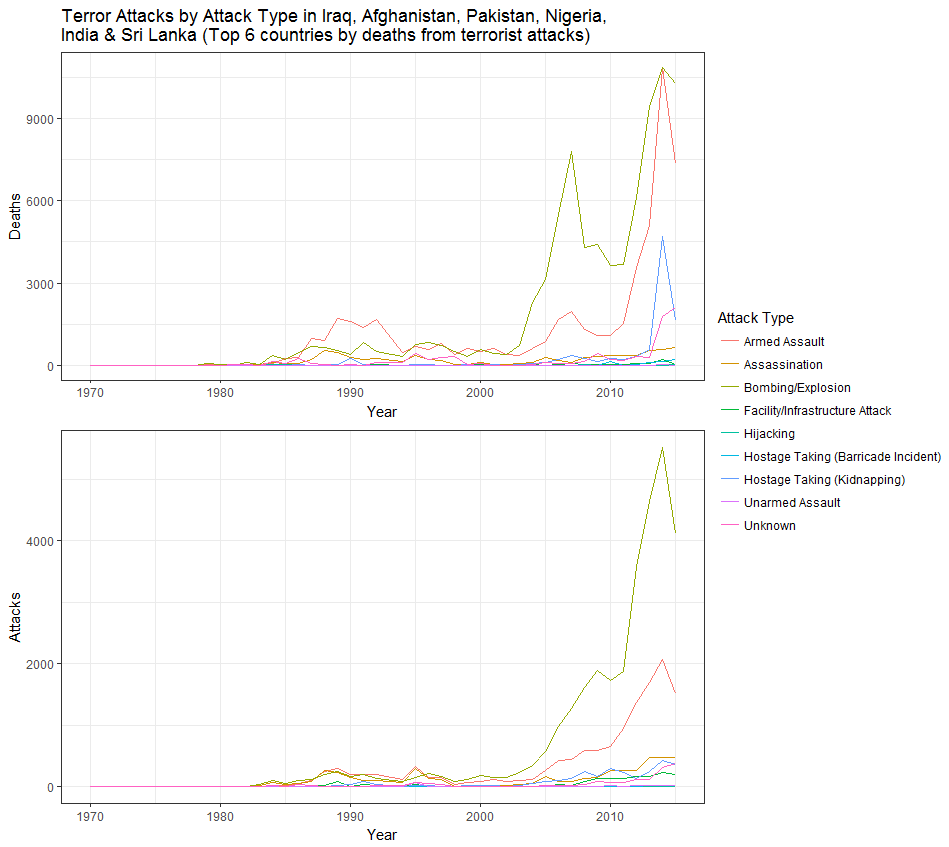
\includegraphics[width=0.8\textwidth]{Plots/AttackType/Top6.png}
	\caption{Terror Attacks by Attack Type in the top six countries by terrorism related deaths (Iraq, Afghanistan, Pakistan, Nigeria, India \& Sri Lanka).}
\end{figure}
\end{center}

\subsection{Terrorism trends over time}
\begin{center}
\begin{figure}[H]
		
	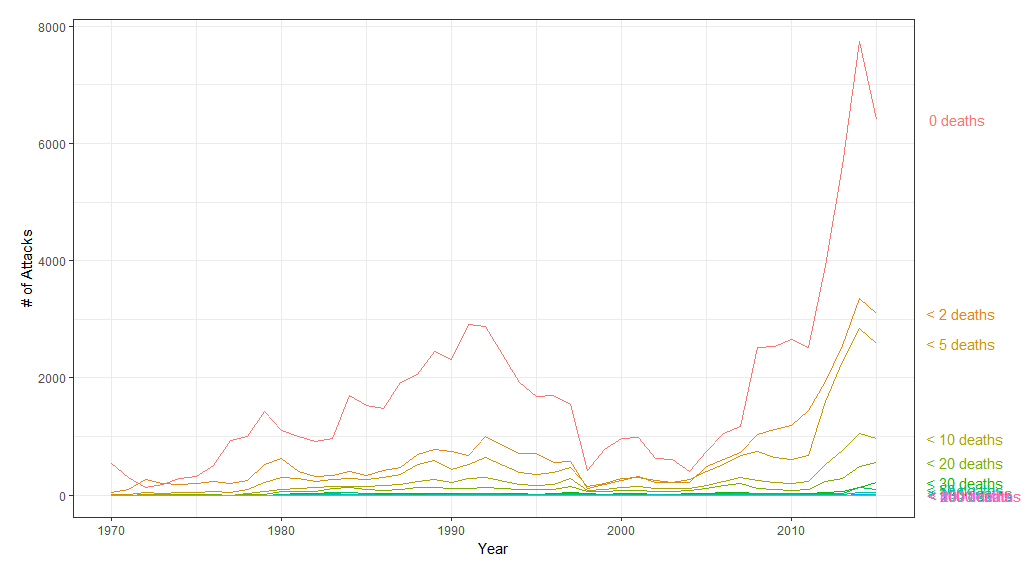
\includegraphics[width=0.8\textwidth]{Plots/OverTime/Attacks_over_time_grouped_by_deaths.png}
	\caption{Number of attacks by year grouped by the number of deaths resulting from the attack.}

\end{figure}
\end{center}

\subsection{Rates of success in terrorist attacks}
\begin{center}
	
\begin{figure}[H]
	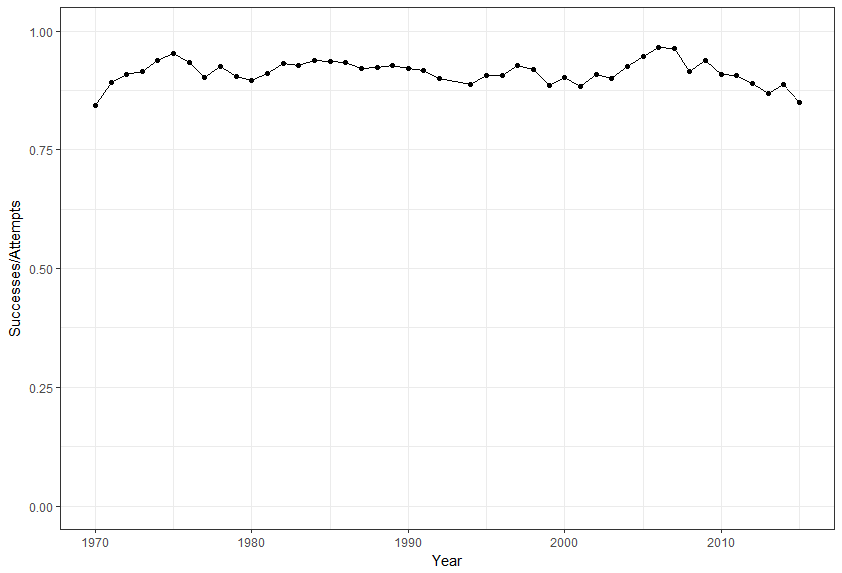
\includegraphics[width=0.8\textwidth]{Plots/OverTime/Successes_vs_Attempts_by_Year.png}
	\caption{Plot of ratio of successful terrorist attacks to total number of attacks globally.}
\end{figure}

\begin{figure}[H]
	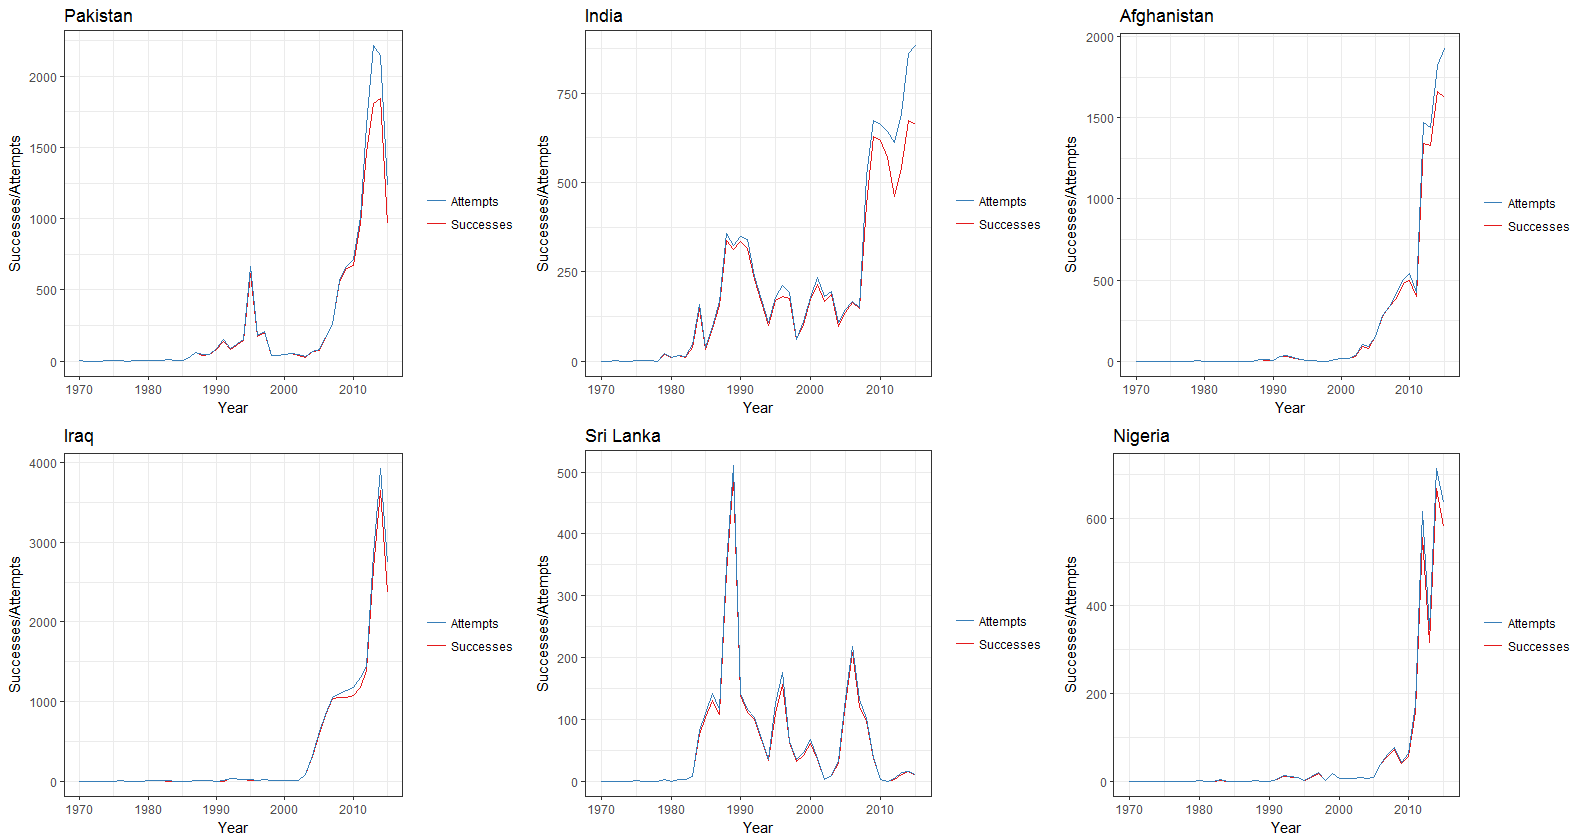
\includegraphics[width=0.8\textwidth]{Plots/OverTime/Top6SuccessVsAttempts.png}
	\caption{Number of successful and total number of attempts plotted by value by year for the Top 6 countries by total deaths as a result of terrorism.}
\end{figure}

\begin{figure}[H]
	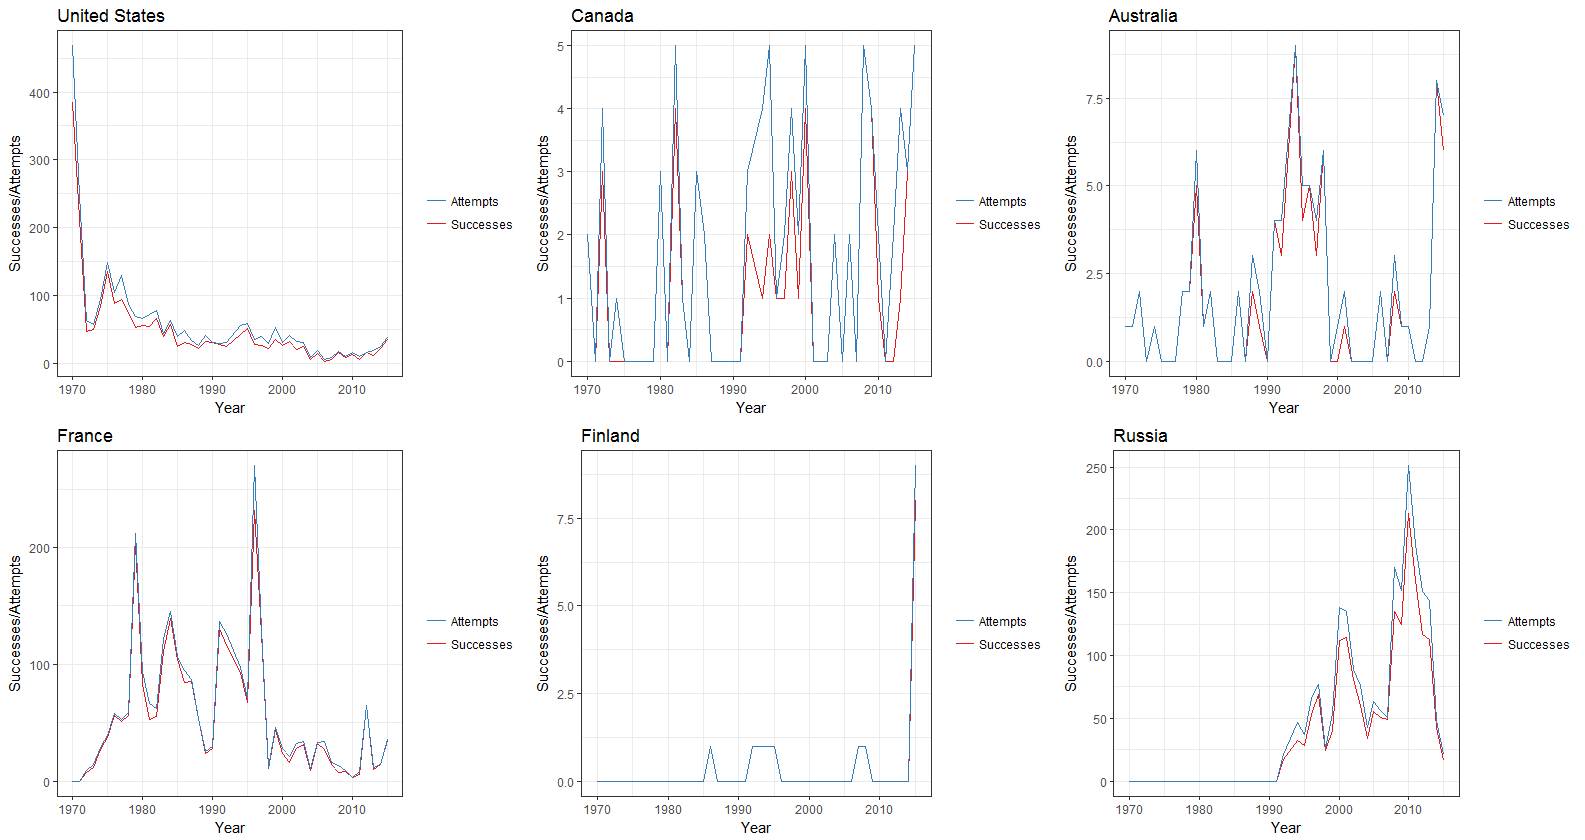
\includegraphics[width=0.8\textwidth]{Plots/OverTime/WesternSuccessVsAttempts.png}
	\caption{Number of successful and total number of attempts plotted by value by year for the six western countries: United states, Canada, Australia, France, Finland and Russia}
\end{figure}
	
\end{center}

\section{Discussion} 

\subsection{Terrorism coverage in United States news data}
The aim in this section is to explore the relationship between terrorist attacks, deaths and media coverage of attacks in the United States. In \textit{Figure 4}, the proportion of terrorism articles to total articles each month has a positive gradient, shown by the fitted robust linear regression model. Although the upwards gradient coefficient is only 0.00037, the proportion of terrorism related articles to total articles is increasing. Between 1970 and September 2001, data fits the linear model quite accurately. In December 2001, the month after \textit{911}, where there was a fatality count of \textit{2997} people, the number of terrorism related articles increases to a proportion of \textit{0.318667236}. In the years following this attack the article ratio converges to the robust linear model.
\\\\
In \textit{Figure 6} we observe an increase in the ratio of terrorism articles to total articles while the number of attacks and deaths decrease. There are numerous possible reasons for this. We speculate the media follows stories of great interest to their readers. Combined with the fear associated with terrorism, terrorism related news articles may increase readership. Additionally the increased perceived threat of terrorism may increase national involvement in the prevention of terrorism.
\\\\
Between 2012 to 2015, there has been a gradual increase in terror related attacks and deaths. This is reflected in the increase in media coverage. 
The correlation coefficients of the number of attacks/deaths and the proportion of terrorism related articles is 0.38 and 0.41 respectively. 
This is representative of some relationship between the number of deaths, attacks and terrorism related articles.
The nature of this relationship is an area of further investigation.
\\\\ 
There is an evident relationship between the number of terrorism related attacks, deaths, and articles over this 45 year time period.
We observe a gradual increase in terror related news articles in recent years, which reflects the slight increase in deaths and attacks as a result of terrorism in the United States over the same time period.
After a large terror event, news related to terrorism not only increases but stays elevated over a prolonged period of time proportional to the impact of the event (here measured in deaths). 
Further investigation is required to determine what relationship exists between the impact of an event and the amount of time the number of terrorism related news article is increased.

\subsection{Methods of Attack}
In this section we explore possible trends in methods of terrorism attacks. Looking at \textit{Figure 10}, there is a great increase in bombing/explosion and armed assault for both death count and attack count but in further analysis, it is seen that these trends are specific to country clusters.
\\\\
In \textit{Figure 8}, the western countries although looking very erratic have a close to consistent ratio of different attack types from 1970 to 2015 for both death count and attack counts. There exists an erratic nature to this graph with no apparent overarching trend. When this is contrasted to \textit{Figure 11}, the 6 countries with highest deaths from terrorist attacks, a number of differences are evident.
\\\\
In the Top six countries bombing/Explosion and armed assault significantly increased from 2000 in the death and attack count. Hostage Taking and unknown increasing from 2003, largely contributing to the death count. 
We speculate that the rise in terrorism related deaths may be the result of numerous reasons: poverty and war-torn regions creating extremists, coupled with new ways to find and recruit extremists. With the increased use of technology and the accessibility of secure messaging and chat rooms may impact the ease of organization of such activities.
\\\\
Further looking at \textit{Figure 7}, the number of attacks has been decreasing since 1970. In \textit{Figure 9}, excluding outliers, the number of deaths resulting from armed assault, bombing/Explosion, and facility/infrastructure attack  has stayed low.
\\\
Each geographical region follows a different trend. Western countries show an erratic and random trend. The Top 6 show a large increase in deaths. The number of attacks in the United States has decreased. Overall, armed assault, bombing/explosion, hijacking and hostage rates taking have increased globally over time, resulting in these attack methods contributing to the most deaths.

\subsection{Terrorism trends over time}

Terrorism trends over time with regard to number of deaths as well as geographical trend visualisations have been conducted in depth in a number of investigations. 
As a result this section of the investigation comprises a small portion of the overall analysis. 
One aspect of the data that was explored was the trends in attacks by the number of deaths as a result of a given attack.
\\\\
The data shown in \textit{Figure 12} shows the number of attacks over time grouped by the number of people killed globally. 
This plot however does not accurately represent the number of people killed over the same time period, since this only looks at numbers of attacks of a certain magnitude in comparison to the number of deaths in total over some time period.
Additionally this does not take into account the number of injuries as a result of these attacks. 
Despite this, we notice a distinct trend. 
\\\\
The majority of attacks over the entire time period are attacks where nobody dies. 
With a total of 70947 attacks (53.02\%) with no deaths over the entire time period surpassing the number of attacks with only one death, which respectively comprised 27988 attacks (20.91\%).
Overall 88\% of attacks result in less than 5 deaths. 
97\% of all attacks result in less than 20 deaths.
The mean number of deaths per attack globally is 2.36. 
Ultimately, despite the greatly increasing number of attacks on a global scale, the number of deaths per attack is small. 
Looking only at attacks where one or more people die, we see the mean deaths per attack  increase to 4.92.
\\\\

\subsection{Rates of success in terrorist attacks}
As shown in the \textit{Figure 13}, the rates of success of terrorist attacks do not vary greatly on a global scale. Despite a greatly varying number of attacks and deaths, especially between the two main country clusters investigated (western countries and the top six countries with regard to total deaths as a result of terrorism), countries in these two clusters have very similar rates of success over time. 


\subsubsection{Westernised Countries}
For a sample of 6 western countries: United States, Canada, Australia, France, Finland and Russia; the respective mean success rates over the 45 year period are 0.807, 0.725, 0.869, 0.904, 0.984 and 0.828; an overall mean success rate of 0.853. However these means misrepresent the number of successes and failures comparatively. Finland, with the highest success rate of these countries had a total of 15 terrorist attacks, 14 of which were successful. 
\\\\
Five of the six countries have had years during this period with no terrorist attacks, Canada: 20, Australia: 17, France: 2, Finland: 38, Russia: 22. The United States however, with a comparatively lower mean success rate, has had no years without a terrorist attack. The rate of success in the United States, despite counter-terrorism related government funding having doubled between 2001 and 2013 (Desilver, 2013).
\\\\
The success rate for Australia, Finland and Canada become increasingly random, or in the case of Finland, increasingly high, due to very few attacks. In the United States, there is an overwhelmingly stable rate of success for terrorist attacks over the 45 year period. Despite this, it is evident in \textit{Figure 15} that the ratio of successful attacks to total attacks overall is comparatively high, with a mean of 0.853 as noted previously.
\\\\
Overall, the number of attacks has decreased over 45 years. Between 2010 and 2015 there is a decrease in the number of attempts (251 to 21) and successes (213 to 16). Along with the rate of success decreasing from 0.849 to 0.762. However this decrease, while being of great magnitude, due to the decreased number of attacks may be skewed. Comparatively in 2014, a success rate of 0.896 was observed. As a result, while the number of attacks is decreasing, it can be said that the rate of success for these attacks is not.
\\\\
While the rate of success for attacks in the west does not appear to be changing drastically in both recent years and over the entire relevant time period, the number of attacks in each of the six countries investigated has decreased drastically. Consequently the rate of success is skewed by the total number of attacks yet remains at a significantly high level.

\subsubsection{Top 6 Countries with respect to deaths from terrorist attacks}
The top six countries with respect to deaths from terrorist attacks are decided upon using \textit{Figure 3}, and are subsequently Iraq, Afghanistan, Pakistan, Nigeria, India and Sri Lanka. These countries will be referred to as simply the \textit{Top 6} for the remainder of this section.
\\\\
These countries, chosen for their comparatively high number of deaths due to terrorism, have higher mean success rates over the period of time between 1970 and 2015.
The data in \textit{Figure 14} shows the number of successful attacks as well as the number of total attacks by year for the countries within the \textit{Top 6}. With mean success rates of:
\\\\ 
\indent Pakistan: 0.939\\
\indent India: 0.918\\
\indent Afghanistan: 0.893\\
\indent Iraq: 0.907\\
\indent Sri Lanka: 0.936\\
\indent Nigeria: 0.932\\
\\
An overall mean success rate of 0.922, higher than that in the western countries mentioned by 0.069. In 2010-2015 alone there were 36978 attacks and 32788 successes, an overall mean success rate of 0.887 over the five year period. Comparatively, in western countries over the same time period, despite only 1110 attacks and 936 successes, the success rate was 0.843. The difference in success rates of terrorist attacks in these two country clusters determined by geographical location terrorism related deaths, differs by only 0.044.
\\\\
In the most recent time period (2000-2015) for all of the Top 6 countries excluding Sri Lanka, the number of attacks has rapidly grown. Overall there were 36978 attacks and 32788 successes in this time period. With high attack numbers, we see success rates converge for almost all of the six countries. With the average success rate over the six countries reaching 0.835 in 2015, country specific success rates maintain high mean values over the five year period. With a peak number of attacks for a number of these countries in 2015, we see a drop in the success rate:
\\\\
\indent \indent(Country: five year mean, 2015 success rate - 2015 attack number) \\
\indent Pakistan: 0.873,  0.781 - 1235  \\
\indent India: 0.814, 0.750 - 882 \\
\indent Afghanistan: 0.909, 0.844 - 1926 \\
\indent Iraq: 0.918, 0.862 - 2743 \\
\indent Sri Lanka: 0.844, 0.818 - 11 \\
\indent Nigeria: 0.911, 0.912 - 637 \\
\\
Only Nigeria shows a similar rate of success in 2015 in comparison to their five year average. It is key to note that the number of attacks in 2015 as seen in \textit{Figure 14} is at an all time high for each country. The reason for this is an area for further investigation.

\subsubsection{Conclusion}
Despite the large geographic difference between the \textit{Top 6} and the westernised countries investigated, there remains a very high success rate of terrorist attacks despite fluctuations in the number of attacks as a whole.
In these Western countries alone, we see a high rate of success with minor fluctuations in countries with a large number of attacks such as the United States.
Countries with generally low numbers of terrorist attacks such as Finland and Australia, suffer from extremely high rates of success.
Regardless of the geographic location, the rate of success seems to be significantly high. In both geographic clusters, greater than 0.8 in all countries excluding Canada, which respectively has a mean success rate of 0.725.


\section{Further Work} 
Due to the exploratory nature of this investigation, there are numerous possibilities for future work.
From the conclusions reached in this investigation, further work in the area of deaths and attack rates by country controlled by population is a necessary step to further understand the data.
Two geographic clusters were investigated in this report:
\\\\
\indent Cluster 1 (Western Countries): United States, Canada, Australia, Finland, France and Russia. \\
\indent Cluster 2 (Top 6): Pakistan, India, Afghanistan, Iraq, Sri Lanka and Nigeria.
\\\\
While these clusters were used to determine differences between typically westernised countries and the top six countries with respect to deaths from terrorism, a well defined clustering of countries regarding the variables in this data should be investigated.

\pagebreak
\begin{thebibliography}{9}

\bibitem{1}
National Consortium for the Study of Terrorism and Responses to Terrorism (START). 
(2016). \textit{Global Terrorism Database}[Data file].
Retrieved from https://www.start.umd.edu/gtd

\bibitem{2}
Charters, D. (1989). Terrorism: A survey of recent literature. Conflict Quaterly, 64-84.

\bibitem{3}
Cornell Law. (n.d.). 18 U.S Code. Retrieved from https://www.law.cornell.edu/text/18/2331

\bibitem{4}
CPOST. (2016, June). The Chicago Project on Security and Terrorism. 
Retrieved from University of Chicago: http://cpost.uchicago.edu/

\bibitem{5}
DoD. (2010). DoD Dictionary of Military and Associated Terms. 
Retrieved from http://www.dtic.mil/doctrine/new\_pubs/dictionary.pdf

\bibitem{6}
FBI. (2002). Terrorism 2002 - 2005. 
Retrieved from https://www.fbi.gov/stats-services/publications/terrorism-2002-2005

\bibitem{7}
FEMA. (2013, July 25). Terrorism. 
Retrieved from FEMA.gov: https://www.fema.gov/media-library-data/20130726-1549-20490-0802/terrorism.pdf

\bibitem{8}
Hill, O. (2016). Contra Wars: The CIA and Its Own Definition of Terrorism. Crescast Scientia Journal of history, 55.

\bibitem{9}
LaFree, G. (2010). The Global Terrorism Database: Accomplishments and Challenges. 
Retrieved from Persepectives on Terrorism Vol 4, No 1: http://www.terrorismanalysts.com/pt/index.php/pot/article/view/89/html

\bibitem{10}
LaFree, G., \& Dugan, L. (2004). How does studying terrorism compare to studying crime? 
Retrieved from Terrorism and Counter-Terrorism (Sociology of Crime, Law and Deviance, Volume 5) Emerald Group Publishing Limited, pp.53 - 74: http://www.emeraldinsight.com/doi/pdfplus/10.1108/S1521-6136%282004%290000005006

\bibitem{11}
Lafree, G., \& Dugan, L. (2007). Introducing the Global Terrorism Database. 
Retrieved from Terrorism and Political Violence: https://ccjs.umd.edu/sites/ccjs.umd.edu/files/pubs/FTPV\_A\_224594.pdf

\bibitem{12}
LaFree, G., Dugan, L., \& Scott, J. (2006). Building a Global terrorism Database. 
Retrieved from University of Maryland: https://www.ncjrs.gov/pdffiles1/nij/grants/214260.pdf

\bibitem{13}
Legal Information Institute. (2016). 22 U.S Code. 
Retrieved from Cornell Law School: https://www.law.cornell.edu/uscode/text/22/2656f

\bibitem{14}
Merari, A. (2007, December 21). Academic research and government policy on terrorism. 
Retrieved from Terrorism and Political Violence: http://www.tandfonline.com/doi/abs/10.1080/09546559108427094

\bibitem{15}
Pape, R., Kevin, R., Bauer, V., \& Jenkins, G. (2014, August 11). How to fix the flaws in the Global Terrorism Database and why it matters. Retrieved from New York Times: 

\bibitem{16}
Desilver, D. (2013). \textit{U.S. spends over \$16 billion annually on counter-terrorism}.
Retrieved from http://www.pewresearch.org/fact-tank/2013/09/11/u-s-spends-over-16-billion-annually-on-counter-terrorism/

\end{thebibliography}

\end{document}
